% first example chapter
% @author Jan Robert Rösler 
%
\chapter{Idee}

\section{DroNet ETH Zürich}
\note{Hier wird das DroNet Paper aufgegriffen und die draus entstandeene Idee erläutert}

Die ETH Zürich entwickelte 2018 eine eigene Architektur, mit dem Ziel durch Training auf Fahrbahnbildern eine Drone zu steuern \cite{loquercio2018dronet}. 
Das daraus entstandene, von Aufbau und Größe relativ einfach gehaltene Neuronale Netz, war der Anstoß für diese Arbeit. 

Das Netz, siehe \ref{img:DroNet}, bekommt als Input ein 200x200 Pixel großes Bild in Graustufen, der Output ist ein Lenkwinkel und zusätzlich eine Kollisionswahrscheinlichkeit.

Es stellte sich heraus, dass das Modell hervorragend generalisierte und eine Drohne sicher durch ein Straßenszenario steuern konnte, wobei das Szenario sich deutlich von den gelernten Unterschied. Diese Eigenschaft von \textsc{DroNet} möchte ich mir im folgenden zu Nutze machen und auf dieser Basis ein Steuerungsmodell für ein RC-Fahrzeug entwickeln.

Die HAW nimmt bereits seit einigen Jahren am \glqq Carolo-Cup \grqq{} teil, einem Wettbewerb der Technischen Universität Braunschweig. Hier treten Teams einiger deutscher Hochschulen mit RC-Fahrzeugen (Maßstab 1:10) in verschiedenen Disziplinen des autonomen Fahrens gegeneinander an. Der Wettbewerb findet jährlich in Braunschweig auf einem vorbereiteten Kurs statt.

Zum entwickeln der Fahrzeuge steht an der HAW eine Teststrecke zur Verfügung \note{BILD}, verschiedene Fahrzeugplattformen sind in der Entwicklung.

Eine hauptsächlich von Nils Schönherr und Gunnar Wolfram aufgebaute Plattform, zu sehen in \ref{img:Carolo-Fahrzeug}, dient dieser Arbeit als Testplattform.



Kenn-Daten von DroNet (Berehcnungszeit, Parameter Layer)


Adaption auf das Carolo Cup Fahrzeug

Performance des Netzes in besimmten Metriken ist nicht intzeressant, da es um die Adaption auf Carolo Teststrecke geht.

Fahren auf der Strecke 

\note{Hervorhaben, welche Teile des DroNet Codes ich weiterverwede. Hard Mining, Auswertungsfunktionen, Architektur}

\section{Carolo-Cup}
aufgabenstellung beim carolocp
haus eigene strecke etc

\begin{figure}
	\centering
	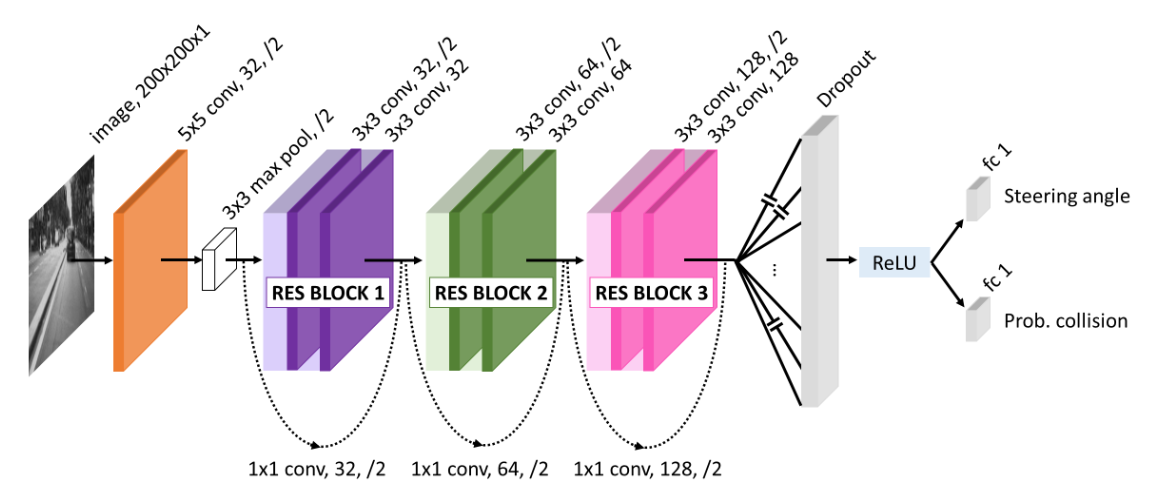
\includegraphics[scale=0.7]{figures/Architecture-DRONET.png}
	\caption{Architektur \textsc{DroNet}}
	\label{img:DroNet}
\end{figure}




\begin{figure}
	\centering
	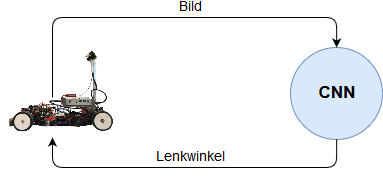
\includegraphics[scale=0.7]{figures/Aufbau.png}
	\caption{Eine tolle Grafik}
	\label{img:toll ist das}
\end{figure}

\section{Die Strecke}

\section{Das Fahrzeug}


\begin{figure}
	\centering
	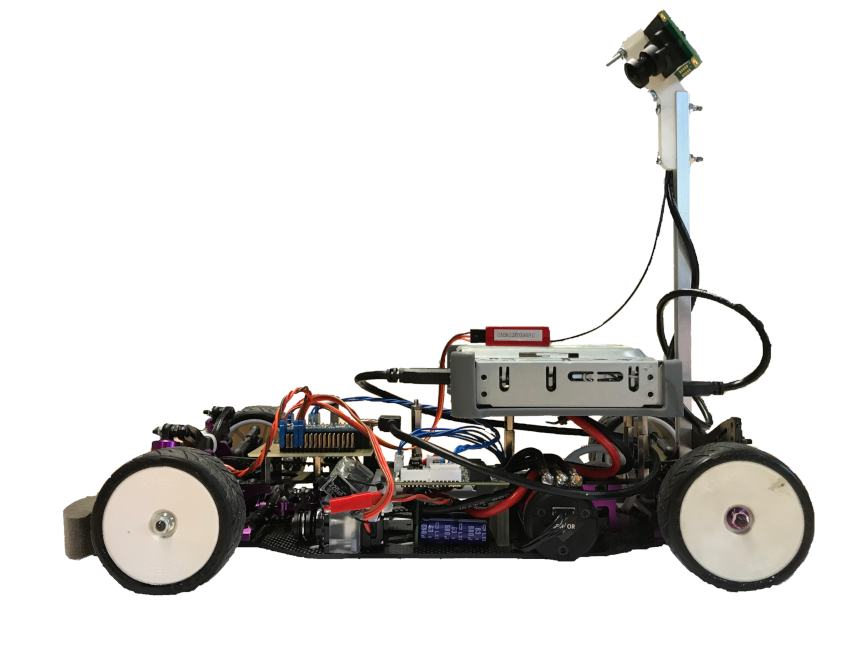
\includegraphics[scale=0.3]{figures/Fahrzeug.png}
	\caption{Das Carolo-Cup Fahrzeug}
	\label{img:Carolo-Fahrzeug}
\end{figure}
